\input{/home/nick/latex-preambles/xelatex.tex}

\newcommand{\imagesPath}{images}

\title{\textbf{Δίκτυα Υπολογιστών} \\~\\Εργαστηριακή Άσκηση 1 \\ Αναλυτής Πρωτοκόλλων Wireshark}
\author{}
\date{}

\begin{document}
	\maketitle
	
	\begin{tabular}{|l|l|}
		\hline
		\textbf{Ονοματεπώνυμο:} Νικόλαος Παγώνας, el18175 & \textbf{Ομάδα:} 4 (Τρίτη εξ' αποστάσεως) \\
		\hline
		\textbf{Όνομα PC/ΛΣ:} nick-ubuntu/Ubuntu 20.04.3 LTS & \textbf{Ημερομηνία:} Τρίτη 12/10/2021  \\
		\hline
		\textbf{Διεύθυνση IP:} \verb|192.168.1.15| & \textbf{Διεύθυνση MAC:} \verb|3c:2c:30:e1:1c:55|\\
		\hline
	\end{tabular}
	
	\subsection*{Άσκηση 1}
	
		\subsubsection*{1.1}
		
		(\textbf{Σημείωση:} Δεν φαίνεται να υπάρχει -προφανής- τρόπος να βρεθεί η ονομασία της κάρτας δικτύου γραφικά, σε περιβάλλον Linux. Επομένως καταφεύγουμε κατευθείαν στο τερματικό.) \\
		
			Με χρήση της εντολής 
				\begin{verbatim}
					lspci | egrep -i --color 'network|ethernet|wireless|wi-fi'
				\end{verbatim}
				
			παίρνουμε το εξής αποτέλεσμα: 
			
			\begin{figure}[H]
				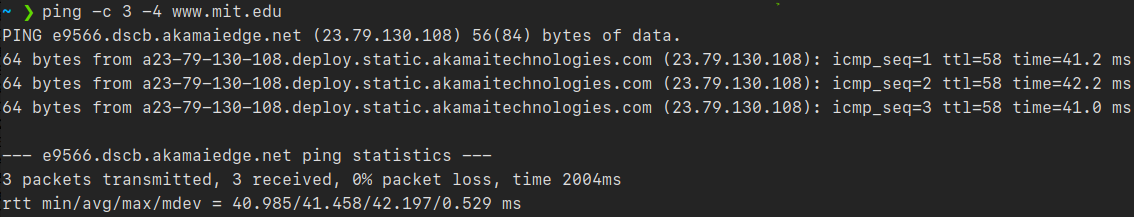
\includegraphics[width=\linewidth]{\imagesPath/1.1.png}	
			\end{figure}
			
			Επιλέγουμε την κάρτα Ethernet (ενσύρματη σύνδεση), καθώς κατά την στιγμή συγγραφής της αναφοράς, είναι ο τρόπος με τον οποίο έχουμε συνδεθεί στο Internet.
		
		\subsubsection*{1.2}
			Όπως προαναφέραμε, η σύνδεση είναι ενσύρματη (Ethernet). 
		
		\subsubsection*{1.3}
			Μέσω του γραφικού περιβάλλοντος επιλέγουμε Settings $\rightarrow$ Network $\rightarrow$ Wired, και πατάμε το εικονίδιο-γρανάζι. 
			Το πεδίο 'Link Speed' μας δείχνει την ταχύτητα της σύνδεσης (100Mbps).
		
		\subsubsection*{1.4}
			Το πεδίο 'Hardware Address' δείχνει την MAC Address (3C:2C:30:E1:1C:55).
		
		\subsubsection*{1.5}
			To πεδίο 'IPv4 Address' δείχνει την IPv4 Address της διεπαφής Ethernet (192.168.1.15)
		
		\subsubsection*{1.6}
			Το πεδίο 'IPv6 Address' δείχνει την IPv6 Address της διεπαφής Ethernet (2a02:587:4511:99f8:48e4:394c:92c4:e992)
		
		\subsubsection*{1.7}
			Το πεδίο 'DNS' δείχνει την διεύθυνση IPv4 του εξυπηρετητή DNS (192.168.1.1)
		
		\subsubsection*{1.8}
			Το πεδίο 'Default Route' δείχνει την διεύθυνση IPv4 της προκαθορισμένης πύλης (192.168.1.1) \\
			
			Τα παραπάνω συνοψίζονται στην εικόνα που ακολουθεί:
			
			\begin{figure}[H]
				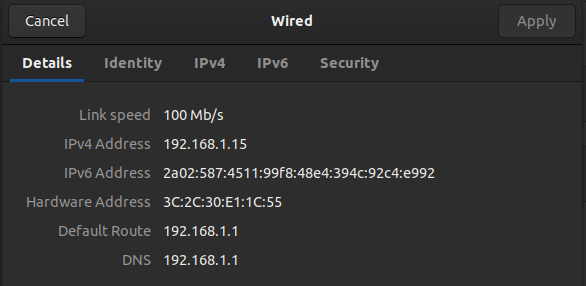
\includegraphics[width=\linewidth]{\imagesPath/1.3.png}
			\end{figure}
		
	\subsection*{Άσκηση 2}
	
		\subsubsection*{2.1}
			Με την εντολή 
			\begin{verbatim}
				hostname
			\end{verbatim}
			
			βρίσκουμε ότι το όνομα του υπολογιστή είναι 'nick-ubuntu'
			
			\begin{figure}[H]
				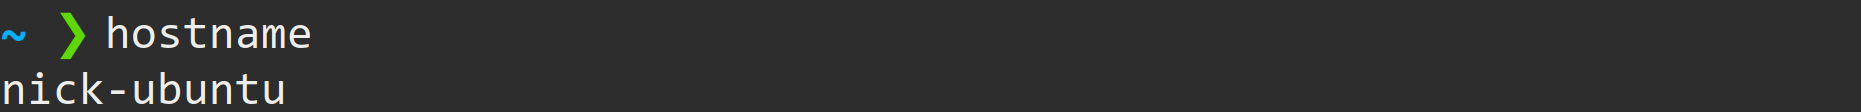
\includegraphics[width=\linewidth]{\imagesPath/2.1.png}
			\end{figure}
			
		\subsubsection*{2.2}
			Μέσω της εντολής:
			\begin{verbatim}
				lscpi | egrep -i --color 'network|ethernet|wireless|wi-fi'
			\end{verbatim}
			
			παίρνουμε και πάλι το εξής αποτέλεσμα: 
			
			\begin{figure}[H]
				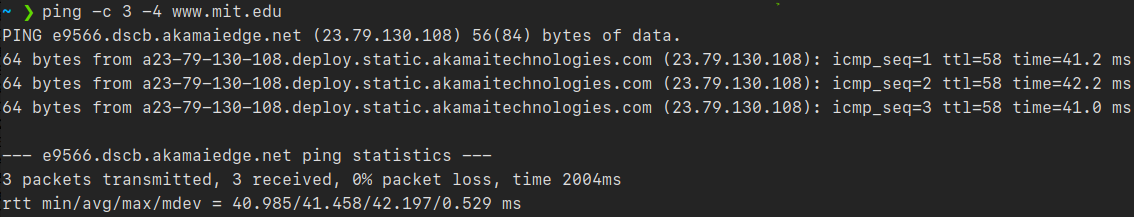
\includegraphics[width=\linewidth]{\imagesPath/1.1.png}
			\end{figure}
		
		\subsubsection*{2.3}
			Με την εντολή 
			\begin{verbatim}
				ifconfig
			\end{verbatim}
			
			παίρνουμε:
			
			\begin{figure}[H]
				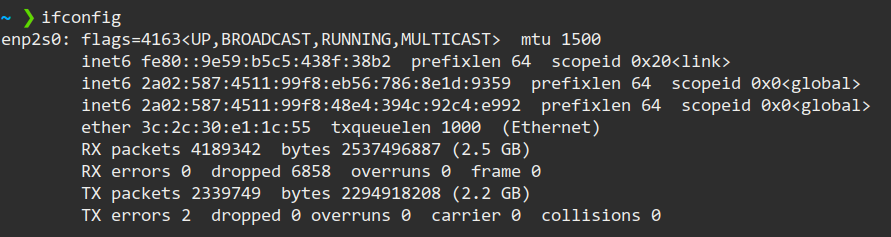
\includegraphics[width=\linewidth]{\imagesPath/2.3.png}
			\end{figure}
		
			Tο πεδίο \verb|ether| δείχνει την MAC Address που ζητείται (3c:2c:30:e1:1c:55). Επιβεβαιώνουμε ότι είναι ίδια με πριν.
		
		\subsubsection*{2.4}
			Με την εντολή 
			
			\begin{verbatim}
				ip addr | grep qlen
			\end{verbatim}
			
			έχουμε:
			
			\begin{figure}[H]
				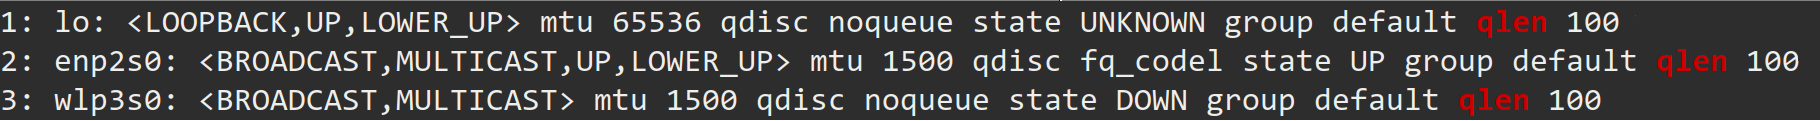
\includegraphics[width=\linewidth]{\imagesPath/2.4.png}
			\end{figure}
		
			όπου σύμφωνα με την τεκμηρίωση του λειτουργικού μας συστήματος, το \verb|qlen| δείχνει την ταχύτητα της σύνδεσης σε Mbps. Άρα, για το interface enp2s0 που μας ενδιαφέρει, η ταχύτητα είναι 100Mbps.
			
		\subsubsection*{2.5}
		
			Με την χρήση της εντολής \verb|ifconfig -a|:
			
			\begin{figure}[H]
				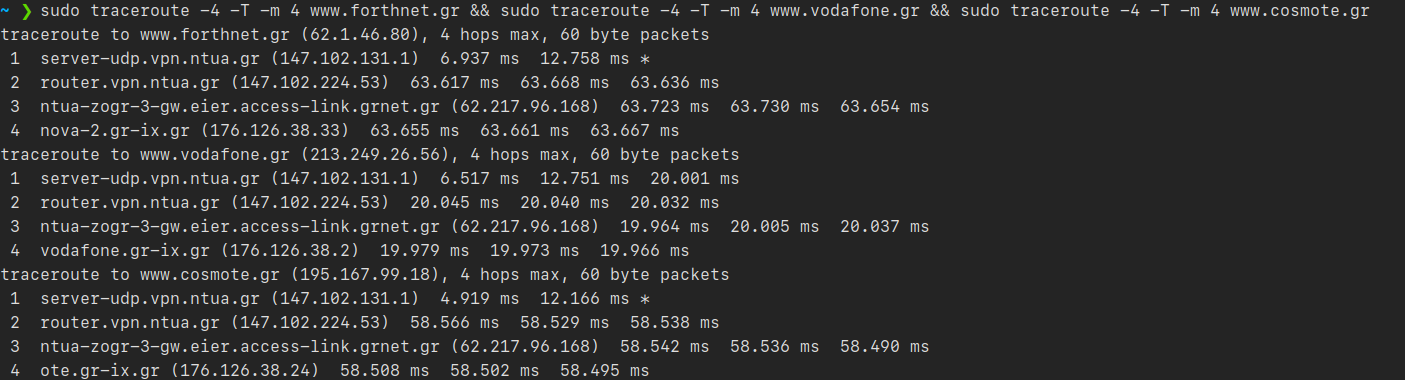
\includegraphics[width=\linewidth]{\imagesPath/2.5.png}
			\end{figure}
		
			Στην δεύτερη γραμμή, βλέπουμε \verb|inet 192.168.1.15|, επομένως αυτή είναι η IPv4 διεύθυνση που ζητείται.
		
		\subsubsection*{2.6}
			Πάλι στην δεύτερη γραμμή, έχουμε \verb|netmask 255.255.255.0|, οπότε αυτή είναι η μάσκα υποδικτύου.
								
			\paragraph{i.}
			
			Αυτό σημαίνει ότι τα 3 πρώτα byte (24 bit) είναι το τμήμα δικτύου ενώ	
			
			\paragraph{ii.}
			
			η διεύθυνση του υποδικτύου είναι \verb|192.168.1.0| (το λογικό AND της μάσκας υποδικτύου με τη διεύθυνση IPv4).
		
		\subsubsection*{2.7}
			Με την εντολή \verb|ip -6 address| έχουμε:
			
			\begin{figure}[H]
				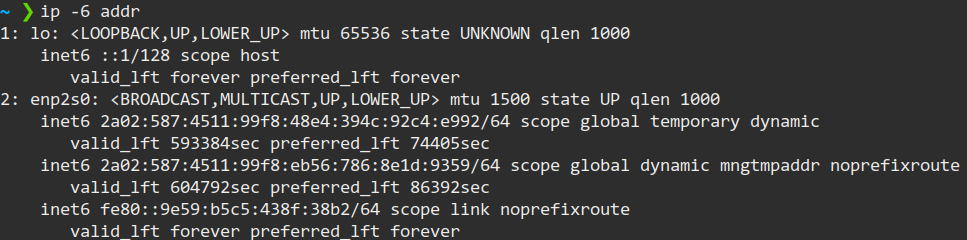
\includegraphics[width=\linewidth]{\imagesPath/2.7.png}
			\end{figure}
		
			οπότε η IPv6 address είναι (2a02:587:4511:99f8:48e4:394c:92c4:e992), η οποία ταυτίζεται με αυτή που βρήκαμε προηγουμένως με γραφικό τρόπο.
			
		\subsubsection*{2.8}
			Με την εντολή \verb+ip route | grep default+ έχουμε: 
		
			\begin{figure}[H]
				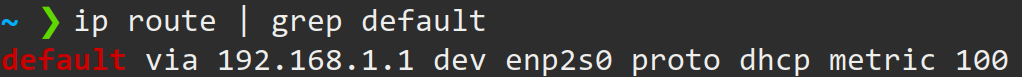
\includegraphics[width=\linewidth]{\imagesPath/2.8.png}
			\end{figure}
		
			από όπου βλέπουμε ότι η IPv4 Address της προκαθορισμένης πύλης είναι 192.168.1.1
		
		\subsubsection*{2.9}
			Με την εντολή \verb|resolvectl| έχουμε:
			
			\begin{figure}[H]
				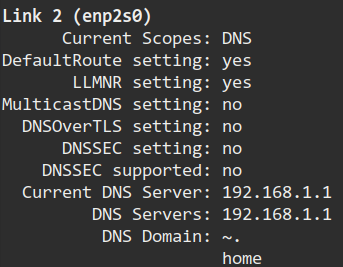
\includegraphics[width=0.5\linewidth]{\imagesPath/2.9.png}
			\end{figure}
		
			οπότε η DNS Server IPv4 Address είναι \verb|192.168.1.1|
			
		\subsubsection*{2.10}
			Με την εντολή \verb|ip route| βλέπουμε:
			
			\begin{figure}[H]
				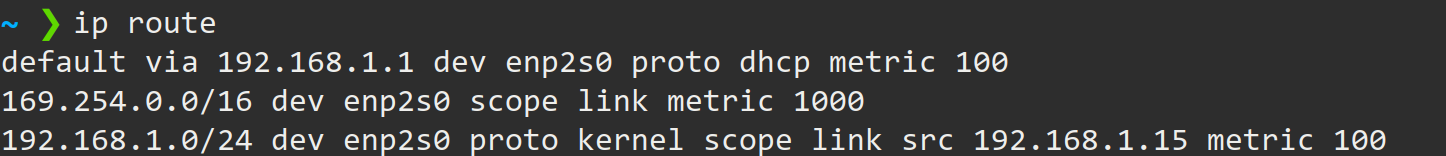
\includegraphics[width=\linewidth]{\imagesPath/2.10.png}
			\end{figure}
		
			και από την πρώτη γραμμή (αναγράφεται το dhcp) βλέπουμε ότι όντως η διεύθυνση του εξυπηρετητή DHCP ταυτίζεται με τον δρομολογητή και είναι η \verb|192.168.1.1|
			
		\subsubsection*{2.11}
		
			Με την εντολή \verb|ip -s link| έχουμε:
			
			\begin{figure}[H]
				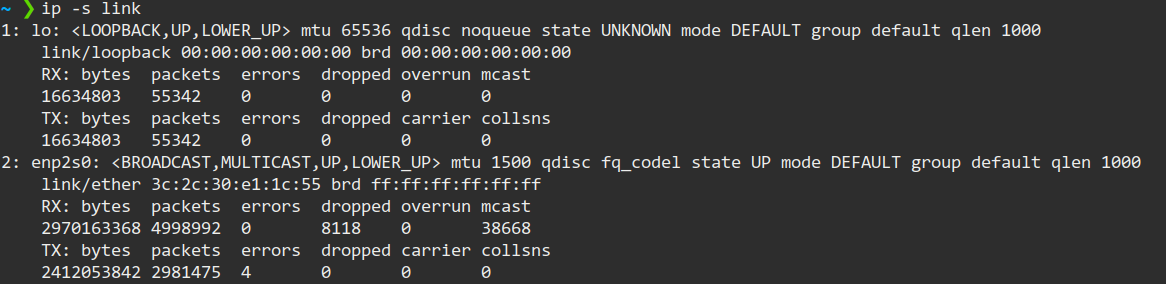
\includegraphics[width=\linewidth]{\imagesPath/2.11.png}
			\end{figure}
		
			Για τη διεπαφή \verb|enp2s0| βλέπουμε: \\
			RX/Received: 2.970.163.368 bytes, 4.998.992 packets \\
			TX/Transmitted: 2.412.053.842 bytes, 2.981.475 packets \\
		
		\subsubsection*{2.12}
		
			Με την εντολή \verb|netstat -s| έχουμε:
			
			\begin{figure}[H]
				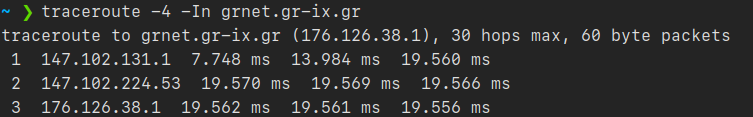
\includegraphics[width=\linewidth]{\imagesPath/2.12.png}
			\end{figure}
			
			Σύμφωνα με το πεδίο "requests sent out", έχουμε 474259 πακέτα που έστειλε η κάρτα δικτύου. Αντίστοιχα, με το πεδίο "incoming packets delivered", έχουμε 961729 πακέτα που έλαβε η κάρτα δικτύου.
				
		\subsubsection*{2.13}
		
			Με την εντολή \verb|ss -n| παίρνουμε μία λίστα των συνδέσεων:
					
			\begin{figure}[H]
				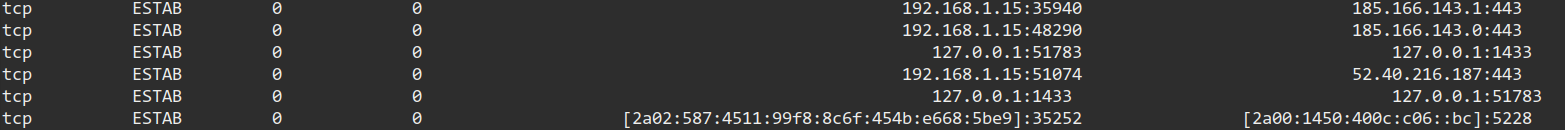
\includegraphics[width=\linewidth]{\imagesPath/2.13.png}
			\end{figure}
		
			Βλέπουμε ότι οι 2 από τις 6 είναι μεταξύ των IP Addresses 127.0.0.1 $\rightarrow$ 127.0.0.1, οπότε οι 4 που απομένουν είναι από τον υπολογιστή μας σε άλλους υπολογιστές.
			
		\subsubsection*{2.14} 
		
			Δύο από αυτές τις συνδέσεις είναι η 1η και 2η στην παραπάνω λίστα, οπότε έχουμε: \\
			Θύρα πηγής $\rightarrow$ 35940 και προορισμού $\rightarrow$ 443. \\
			Θύρα πηγής $\rightarrow$ 48290 και προορισμού $\rightarrow$ 443. \\

	\subsection*{Άσκηση 3}
	
		\subsubsection*{3.1}
			Αφού σταματήσει η καταγραφή, παρατηρούμε ότι εμφανίζονται τα πρωτόκολλα ARP, DNS, HTTP, HomePlug AV, ICMP, ICMP v6, STUN, TCP, TLSv1.2, UDP και ieee1905.
		
		\subsubsection*{3.2}
			Αφού εφαρμόσουμε το φίλτρο \verb|ip.addr==147.102.40.15| και επιλέξουμε το πρώτο μήνυμα HTTP με εντολή GET, έχουμε την εξής εικόνα:
			
			\begin{figure}[H]
				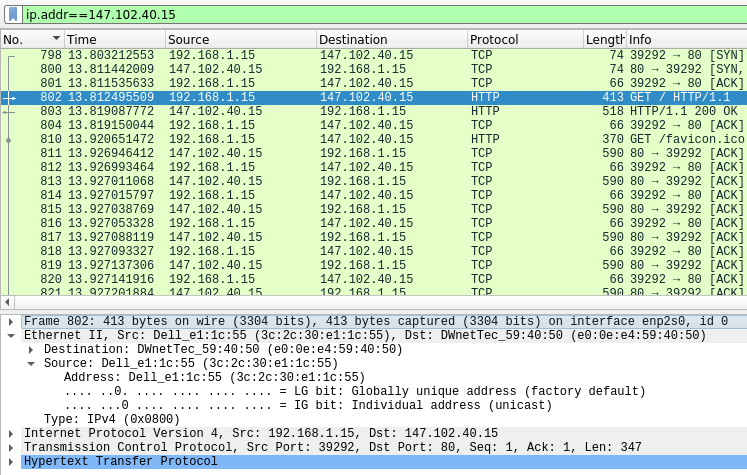
\includegraphics[width=\linewidth]{\imagesPath/3.2.png}
			\end{figure}
		
		Παρατηρώντας την επικεφαλίδα του πλαισίου Ethernet, βλέπουμε 
		\begin{verbatim}
			Src: Dell_e1:1c:55 (3c:2c:30:e1:1c:55)
		\end{verbatim}
		
		Η MAC Address του υπολογιστή μας είναι αυτή που βρίσκεται μέσα στην παρένθεση.
		
		\subsubsection*{3.3}
			Από το παραπάνω, βλέπουμε ότι ο κατασκευαστής της κάρτας δικτύου είναι η DELL.
		
		\subsubsection*{3.4}
			Εξακολουθώντας να βλέπουμε το πλαίσιο που αφορά το μήνυμα HTTP GET, από την επικεφαλίδα του πλαισίου "Internet Protocol Version 4":
			
			\begin{figure}[H]
				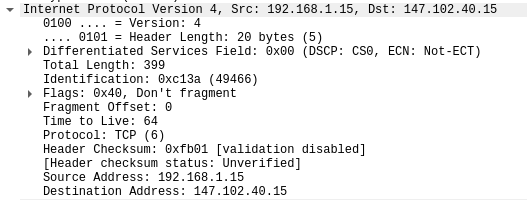
\includegraphics[width=\linewidth]{\imagesPath/3.4.png}
			\end{figure}
		
			βλέπουμε 
			
			\begin{verbatim}
				Src: 192.168.1.15
			\end{verbatim}
		
		οπότε η διεύθυνση IPv4 του υπολογιστή μας είναι η παραπάνω.
		
		\subsubsection*{3.5}
			Από την ίδια επικεφαλίδα βλέπουμε
			
			\begin{verbatim}
				Dst: 147.102.40.15
			\end{verbatim} 
		
		οπότε η διεύθυνση IPv4 του edu-dy.cn.ntua.gr είναι η παραπάνω (η ίδια που έχουμε βάλει στο φίλτρο απεικόνισης).
		
		\subsubsection*{3.6}
			Η σύνταξη του φίλτρου είναι τώρα: \verb|tcp.stream eq 15|
					
		\subsubsection*{3.7}
		
			Τα αποτελέσματα της προηγούμενης καταγραφής είναι τα εξής:
		
			\begin{figure}[H]
				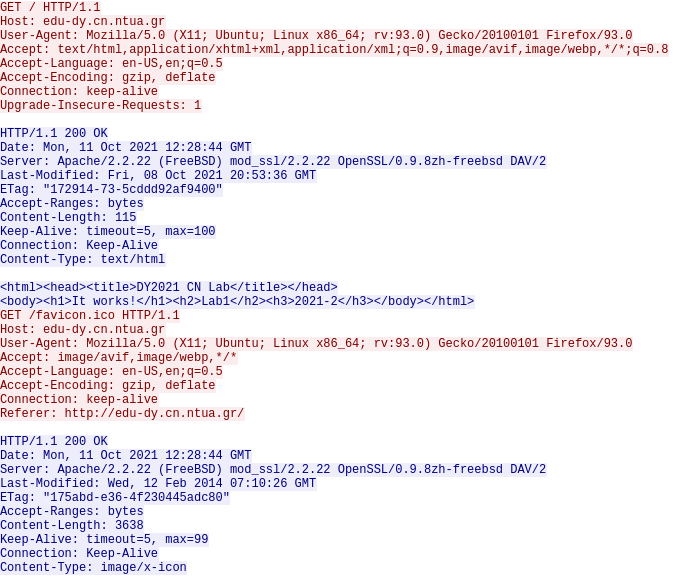
\includegraphics[width=\linewidth]{\imagesPath/3.7.png}
			\end{figure}
			
			Έτσι, βλέπουμε ότι:
			
			\paragraph{i.}
				Ο εξυπηρετητής ιστού που φιλοξενεί τη σελίδα που επισκεφθήκαμε είναι Apache:
				
				\begin{verbatim}
					Server: Apache/2.2.22 (FreeBSD) mod_ssl/2.2.22 OpenSSL/0.9.8zh-freebsd DAV/2
				\end{verbatim} 		
				
			\paragraph{ii.}
				Ο τίτλος της σελίδας είναι \textbf{DY2021 CN Lab} (το κομμάτι που φαίνεται ο τίτλος στην HTML είναι υπογραμμισμένο με "====")
				
				\begin{verbatim}
					<html><head><title>DY2021 CN Lab</title></head>
					            ============================
					<body><h1>It works!</h1><h2>Lab1</h2><h3>2021-2</h3></body></html>
				\end{verbatim}
				
			
			\paragraph{iii.}
				Ο τίτλος φαίνεται στην καρτέλα/tab του φυλλομετρητή που αντιστοιχεί στη σελίδα που επισκεφθήκαμε.
				
				\begin{figure}[H]
					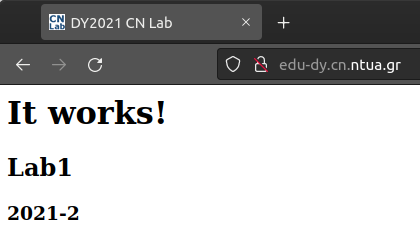
\includegraphics[width=\linewidth]{\imagesPath/3.7.iii.png}
				\end{figure}
		
		\subsubsection*{3.8}
			Με το φίλτρο \verb|http| εμφανίζουμε μόνο τα HTTP μηνύματα. 
			
			\begin{figure}[H]
				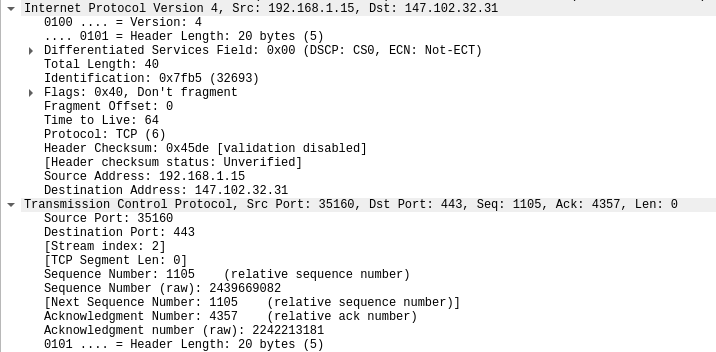
\includegraphics[width=\linewidth]{\imagesPath/3.8.png}
			\end{figure}
			
		
		\subsubsection*{3.9}
			Παρατηρούμε ότι υπάρχουν 4 HTTP μηνύματα, όλα μεταξύ των διευθύνσεων IP που προαναφέραμε. Από αυτά, 2 έχουν σταλεί (αυτά με μήνυμα GET), και 2 έχουν ληφθεί (αυτά με μήνυμα 200 OK).
		
		\subsubsection*{3.10}
			Με την επιλογή View $\rightarrow$ Time Display Format $\rightarrow$ Seconds Since Previous Displayed Packet μπορούμε να δούμε κατευθείαν πόσος χρόνος πέρασε μεταξύ μόνο των πακέτων που μας ενδιαφέρουν.
			
			\begin{figure}[H]
				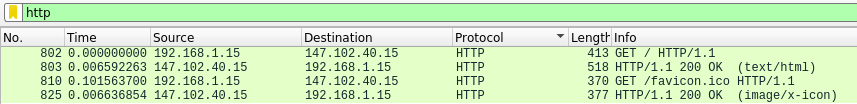
\includegraphics[width=\linewidth]{\imagesPath/3.10.png}
			\end{figure}
		
			Έτσι, βλέπουμε ότι ο χρόνος που πέρασε από την στιγμή που στάλθηκε το πρώτο αίτημα GET μέχρι να ληφθεί η απόκριση 200 OK είναι 6.6 msec.
			
		\subsubsection*{3.11}
		
			Στο πεδίο "Reassembled TCP Segments" βλέπουμε ότι χρειάστηκαν 8 πακέτα για την ολοκλήρωση της μετάδοσης.
		
			\begin{figure}[H]
				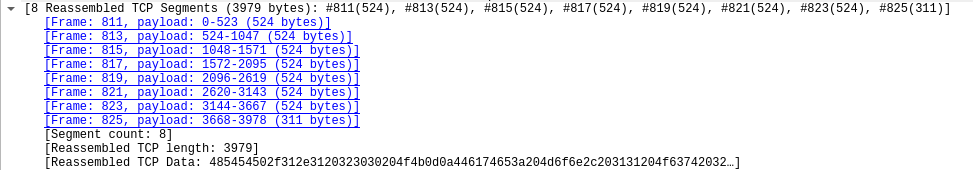
\includegraphics[width=\linewidth]{\imagesPath/3.11.png}
			\end{figure}
		
		\subsubsection*{3.12}
		
			Κρατάμε μόνο το φίλτρο για την διεύθυνση \verb|147.102.40.15| και μας ενδιαφέρουν τα πακέτα 811, 813, 815, 817, 819, 821, 823, 825.
			
			\begin{figure}[H]
				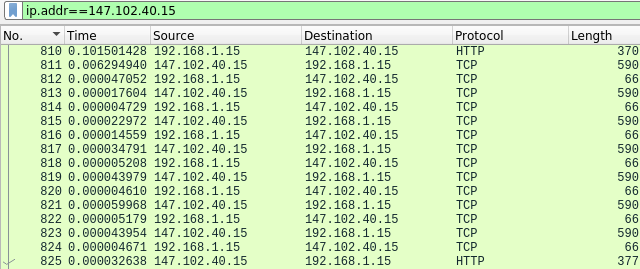
\includegraphics[width=\linewidth]{\imagesPath/3.12.png}
			\end{figure}
		
			Βλέπουμε ότι το πρώτο πακέτο (811) έκανε 6.3 msec να ληφθεί (από την στιγμή που εστάλη το HTTP GET Request).
			Αν αθροίσουμε όλους τους χρόνους των επόμενων πακέτων, βρίσκουμε ότι χρειάστηκαν επιπλέον 0.3 msec για υπόλοιπα, ενώ για την απόκριση στο αίτημα GET χρειάστηκαν επιπλέον 0.03 msec, άρα συνολικά 6.63 msec.
		
		
		\subsubsection*{3.13}
			Οι χρόνοι που προκύπτουν είναι οι εξής:
		
			\begin{verbatim}
				[Service Time: 0.006294940 seconds]
				[Rsp Spread: 0.000341914 seconds]
				[APDU Rsp Time: 0.006636854 seconds]
			\end{verbatim}
			
			Παρατηρούμε ότι είναι αντίστοιχοι αυτών που υπολογίσαμε χειροκίνητα προηγουμένως.
			
		\subsubsection*{3.14}	
			Με την εντολή \verb|ip.src == 192.168.1.15 && http| μπορούμε να δούμε μόνο τα μηνύματα HTTP που έστειλε ο υπολογιστής μας.
			
			\begin{figure}[H]
				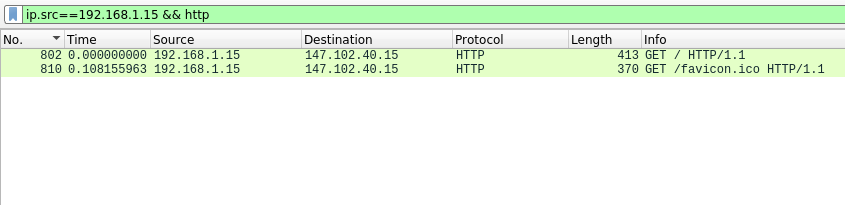
\includegraphics[width=\linewidth]{\imagesPath/3.14.png}
			\end{figure}
\end{document}